\documentclass[12pt]{article}
\usepackage{amsmath, amsthm, amssymb}
\usepackage{hyperref}
\usepackage{booktabs}
\usepackage{geometry}
\geometry{margin=1in}

\newtheorem{conjecture}{Conjecture}
\newtheorem{theorem}{Theorem}
\newtheorem{proposition}{Proposition}
\newtheorem{remark}{Remark}

\title{Structural Conjectures for $4 \times n$ Chomp:\\
Unique Extension, Asymptotic Ratios, and Period-112 Geometry}

\author{Arnav Garg \\
\small BITS Pilani, Pilani Campus \\
\small \texttt{gargarnav2007@gmail.com}}

\date{\today}

\begin{document}
\maketitle

\begin{abstract}
We present a computational study of P-positions (losing positions for
the player to move) in $4 \times n$ Chomp, the combinatorial game
played on a $4 \times n$ rectangular grid. Using an optimized C++
solver with bitpacked state representation, we tabulate all 4,316,097
P-positions for boards with $n \leq 500$, constituting the most
extensive computational study of $4 \times n$ Chomp to date.
Our analysis reveals four structural conjectures: (1) a \emph{Unique
Extension} property, stating that for any triple $(a,b,c)$ of row
lengths, there is at most one valid fourth-row length $d$ completing
a P-position; (2) convergence of row-length ratios to fixed asymptotic
constants; (3) a period-112 modular structure governing the set of
extendable triples; and (4) a linear cone geometry for the P-position
set in $(a,b,c)$-space. These findings suggest a richer deterministic
structure in $4 \times n$ Chomp than previously suspected and raise
new questions about the relationship between $k$-row games for
consecutive $k$.
\end{abstract}

%%% SECTION 1: INTRODUCTION
\section{Introduction}

Chomp is a two-player combinatorial game introduced by David Gale
\cite{gale1974} and popularized by Martin Gardner \cite{gardner1973}.
The game is played on an $m \times n$ rectangular grid of squares.
Players alternate turns; on each turn, a player selects any remaining
square and removes it together with all squares above and to the right.
The square at position $(1,1)$ (the top-left corner) is \emph{poisoned}:
whoever is forced to take it loses.

A strategy-stealing argument establishes that the first player wins on
any board larger than $1 \times 1$: if the second player had a winning
strategy $\sigma$, the first player could take only the bottom-right
square and then adopt $\sigma$, contradicting the assumption
\cite{berlekamp2001}. This non-constructive argument gives no
information about the winning move or the structure of losing positions
(P-positions).

The complete structure of Chomp P-positions is known only for special
cases:
\begin{itemize}
  \item $1 \times n$: trivially solved (take all but the poison square).
  \item $2 \times n$: fully solved; the P-positions are exactly the
        positions $(a, a-1)$ for $a \geq 1$ \cite{berlekamp2001}.
  \item $n \times n$ (square boards): the first player always wins by
        taking position $(2,2)$ and maintaining symmetry.
  \item $3 \times n$: Zeilberger \cite{zeilberger2001} computed all
        P-positions up to $n = 130{,}000$ and found apparent periodic
        structure, later studied by Brouwer et al.\ \cite{brouwer2005},
        who gave a cubic-time algorithm and proved infinitely many
        winning first moves exist in the third row.
\end{itemize}

The $4 \times n$ case has received no systematic computational treatment.
We address this gap. Our main contribution is a complete tabulation of
$4 \times n$ P-positions for $n \leq 500$ and the identification of
four structural conjectures, the most striking of which is:

\begin{conjecture}[Unique Extension]
For any triple of non-negative integers $(a, b, c)$ with $a \geq b
\geq c \geq 0$, there exists \emph{at most one} non-negative integer
$d$ such that $(a, b, c, d)$ is a P-position of $4 \times n$ Chomp.
\end{conjecture}

This property, verified for all 4,316,097 P-positions with $n \leq 500$,
suggests that the $4$-row game is in a precise sense a ``deterministic
lift'' of the $3$-row game: the fourth coordinate is uniquely determined
by the first three.

%%% SECTION 2: SETUP AND SOLVER
\section{Computational Setup}

\subsection{State Representation}

A position in $4 \times n$ Chomp is fully described by a non-increasing
tuple $(a, b, c, d)$ of non-negative integers with $a \geq b \geq c
\geq d \geq 0$, where each coordinate gives the number of remaining
squares in the corresponding row. The initial position of a $4 \times n$
board is $(n, n, n, n)$, and the unique terminal P-position is
$(1, 0, 0, 0)$ (only the poisoned square remains).

\subsection{Solver Algorithm}

We implemented a retrograde solver in C++ using the following design
decisions:
\begin{enumerate}
  \item \textbf{Bitpacked states}: Each tuple $(a,b,c,d)$ is encoded
        as a single \texttt{uint64\_t} with four 16-bit fields, enabling
        fast hashing and minimal memory footprint.
  \item \textbf{Sparse storage}: Only P-positions (a small fraction of
        all states) are stored in a hash set. N-positions are not stored;
        the solver short-circuits as soon as any move to a P-position
        is found.
  \item \textbf{Bottom-up evaluation}: States are evaluated in increasing
        order of total cell count, ensuring all successors are resolved
        before each state is evaluated.
\end{enumerate}

The solver tabulated all P-positions for $n \leq 500$ in approximately
70 minutes on an Apple M4 processor with 24~GB RAM, using at most 45~MB
of memory.

\subsection{Verification}

We verified the solver output against two known ground truths:
\begin{enumerate}
  \item \textbf{$2 \times n$ subcase}: All P-positions with $c = d = 0$
        satisfy $(a, b, 0, 0) = (a, a-1, 0, 0)$ for all $a \geq 1$,
        matching the known formula exactly.
  \item \textbf{$3 \times n$ subcase}: An independent memoized Python
        solver verified all P-positions with $d = 0$ up to $n = 50$
        against the $4 \times n$ output; no discrepancies were found.
  \item \textbf{Data correction}: A hidden 5th column in the raw CSV output
        caused a column-shift bug in early analysis. All results presented
        here use the corrected mapping, verified by cross-checking the
        $d=0$ subcase and the $c=d=0$ subcase.
\end{enumerate}

\begin{table}[h]
\centering
\caption{First 10 P-positions of $4 \times n$ Chomp
         (lexicographic order by $(a,b,c)$)}
\begin{tabular}{rrrr}
\toprule
$a$ & $b$ & $c$ & $d$ \\
\midrule
 1 & 0 & 0 & 0 \\
 2 & 1 & 0 & 0 \\
 2 & 2 & 1 & 0 \\
 2 & 2 & 2 & 1 \\
 3 & 1 & 1 & 0 \\
 3 & 2 & 0 & 0 \\
 3 & 3 & 1 & 1 \\
 4 & 1 & 1 & 1 \\
 4 & 2 & 2 & 0 \\
 4 & 3 & 0 & 0 \\
\bottomrule
\end{tabular}
\label{tab:first10}
\end{table}

The lexicographical sequence of $d$-values begins:
\texttt{0, 0, 0, 1, 0, 0, 1, 1, 0, 0, 1, 0, 2, 0, 2, 0, 2, 0, 0, 0, 2, 0, 2, 0, 2, 3, 4, 0, 3, 0}.

%%% SECTION 3: MAIN CONJECTURES
\section{Main Conjectures}

\subsection{Conjecture 1: Unique Extension}

\begin{conjecture}[Unique Extension]
\label{conj:unique}
For any triple $(a, b, c)$ with $a \geq b \geq c \geq 0$, there exists
at most one non-negative integer $d$ such that $(a, b, c, d)$ is a
P-position of $4 \times n$ Chomp.
\end{conjecture}

\begin{remark}
Equivalently, the projection map $\pi: (a,b,c,d) \mapsto (a,b,c)$
is injective on the set of $4 \times n$ P-positions. This does not
hold for all three-element projections: multiple $(a,b,c,d)$ may share
the same $(b,c,d)$ triple.
\end{remark}

\noindent\textbf{Evidence.} We tested Conjecture~\ref{conj:unique} on
all 4,316,097 P-positions computed for $n \leq 500$. For each distinct
triple $(a,b,c)$ appearing as a prefix, we counted the number of valid
extensions $d$. In every case, exactly one extension was found. No
violation was detected.

Note that not every triple $(a,b,c)$ extends: approximately 20\% of all
valid triples with $a \leq 500$ appear as prefixes of P-positions.
Every known $3 \times n$ P-position $(a,b,c)$ is among this 20\%,
but the converse fails --- the majority of extending triples are
$3 \times n$ N-positions.

\subsection{Conjecture 2: Asymptotic Ratios}

\begin{conjecture}[Asymptotic Ratios]
\label{conj:ratios}
For P-positions $(a, b, c, d)$ of $4 \times n$ Chomp with $a$ large,
the row-length ratios converge to fixed constants:
\[
\frac{b}{a} \to L_1 \approx 0.762, \quad
\frac{c}{a} \to L_2 \approx 0.499, \quad
\frac{d}{a} \to L_3 \approx 0.224,
\]
as $a \to \infty$.
\end{conjecture}

\begin{figure}[h]
\centering
%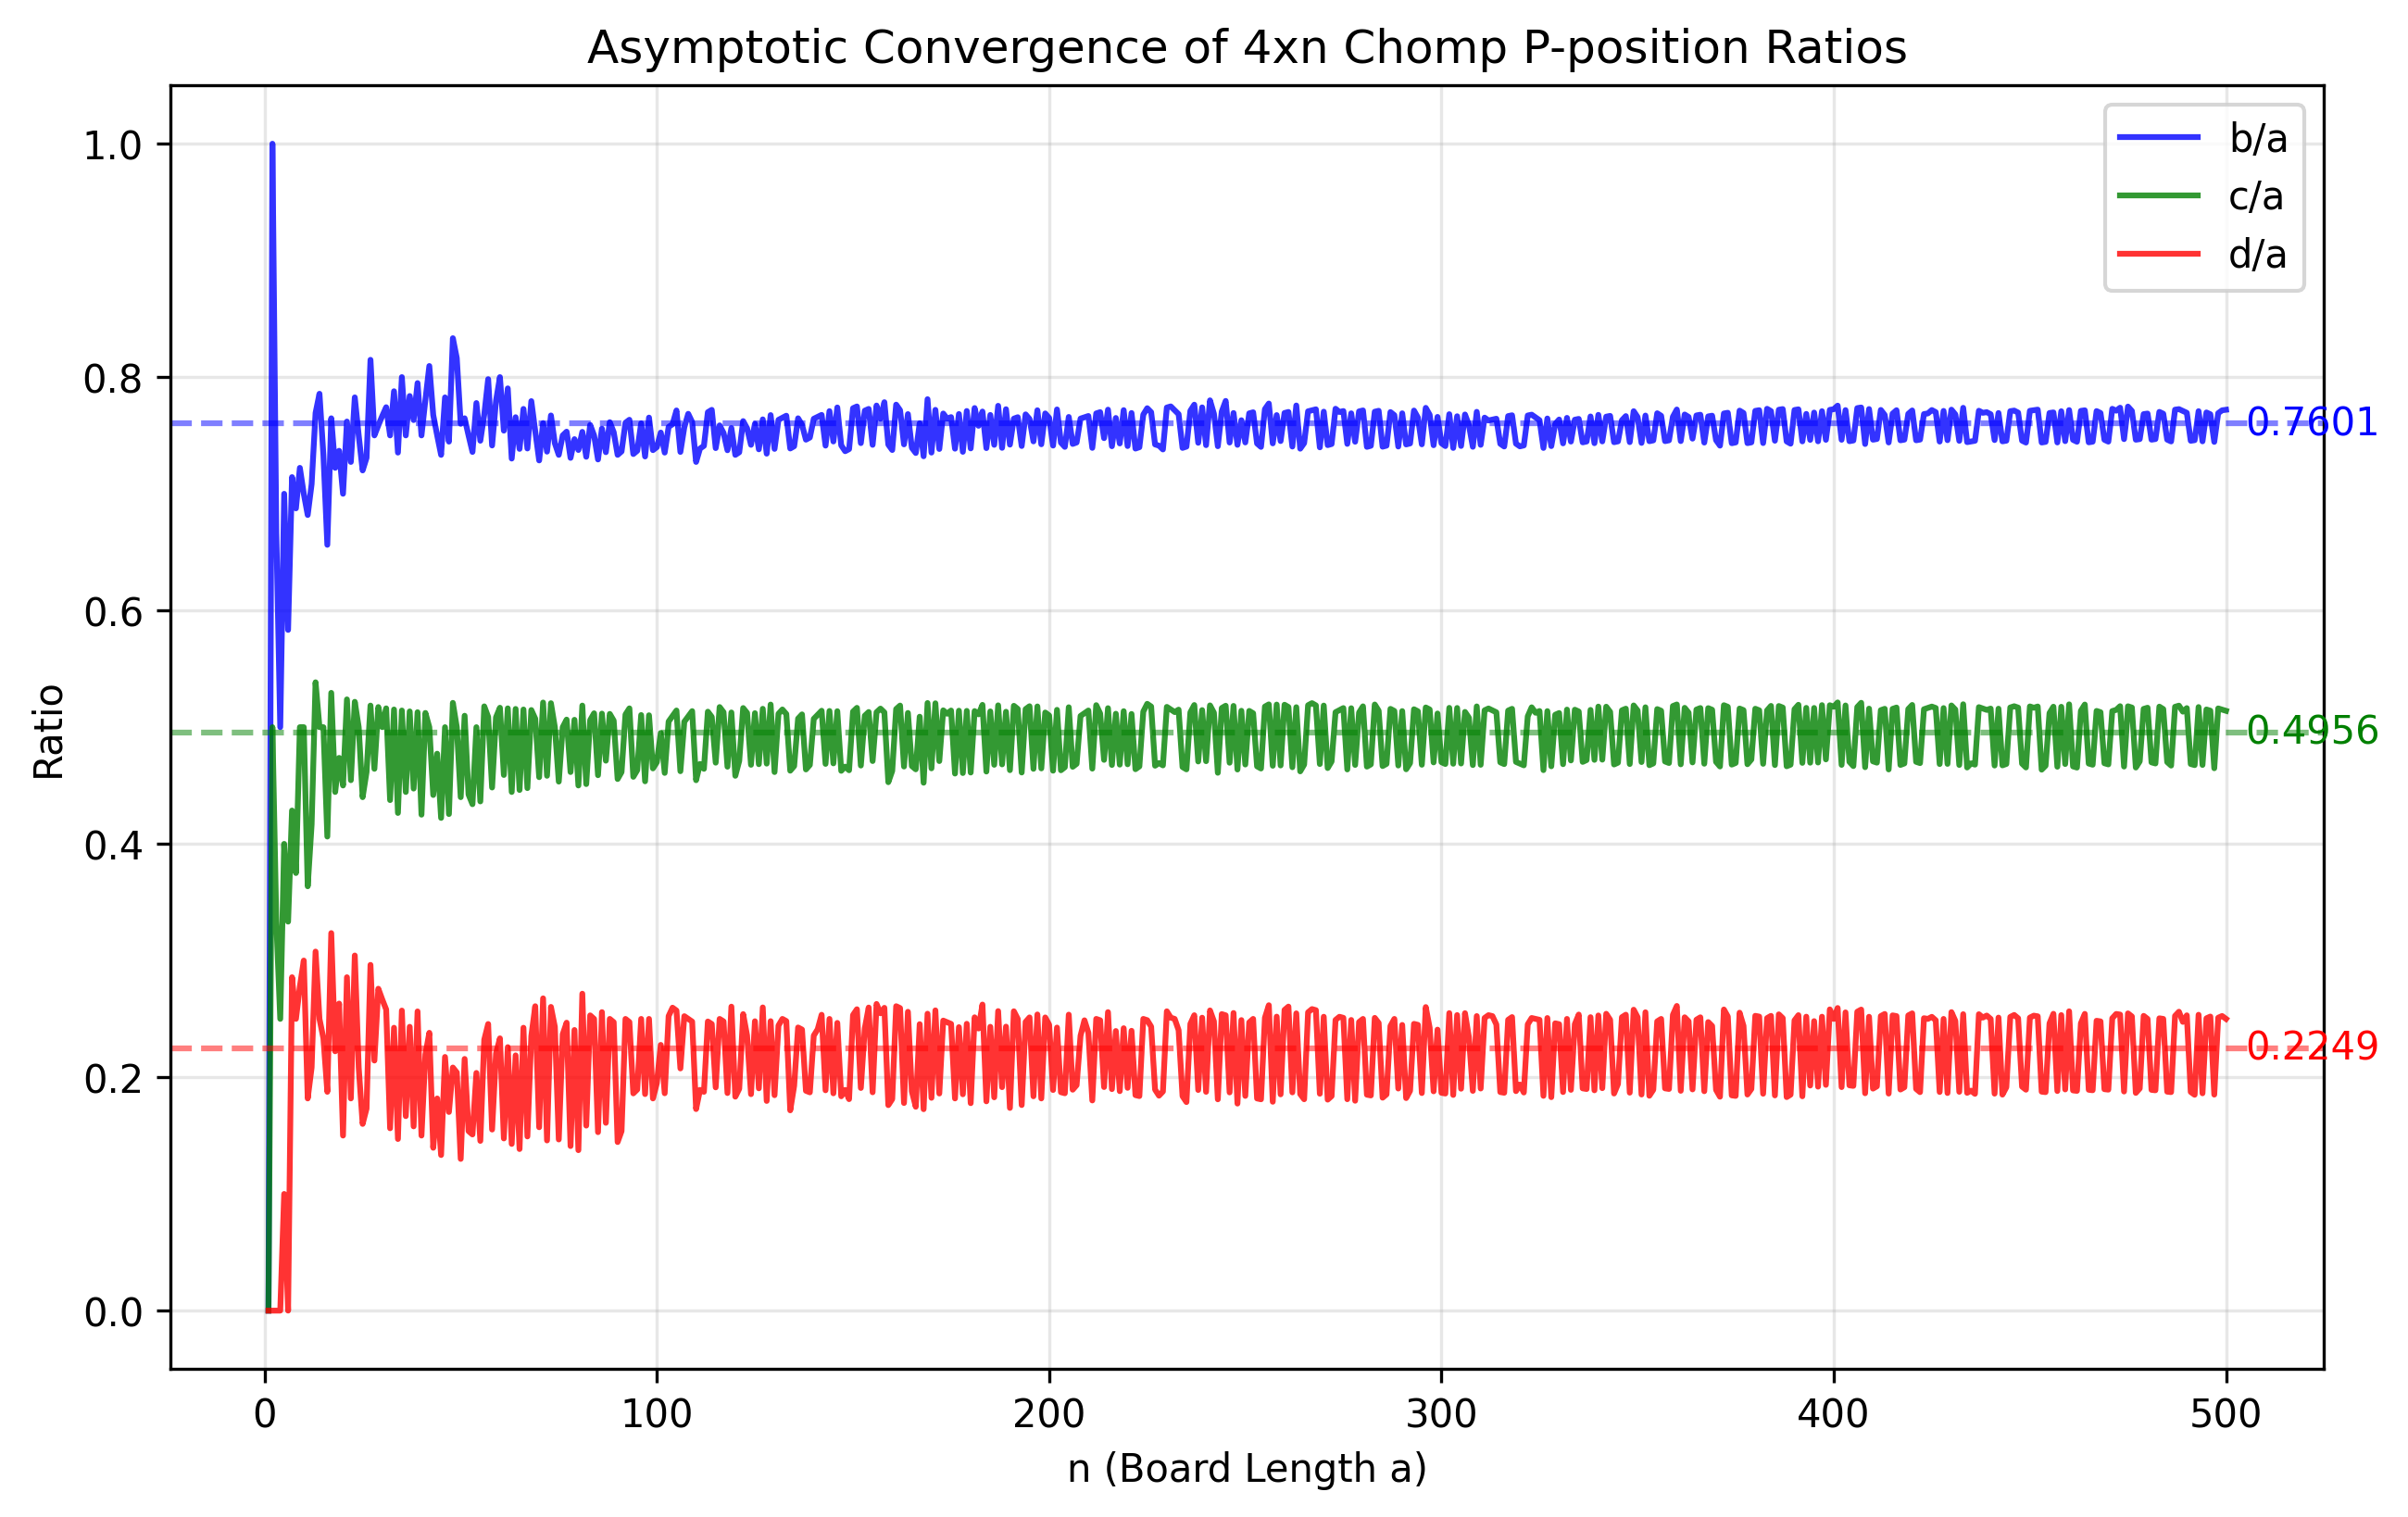
\includegraphics[width=0.85\textwidth]{figures/fig2_ratio_convergence.png}
\caption{Convergence of row-length ratios $b/a$, $c/a$, $d/a$ for
         P-positions with $n \leq 500$. Solid lines show windowed
         medians; dashed lines show conjectured limit values.}
\label{fig:ratios}
\end{figure}

These values were estimated by three independent methods (windowed
median for $a > 450$, rolling window, and power-law curve fitting
$L + Ka^{-p}$) applied to the $n \leq 500$ dataset. $L_2$ and $L_3$
are stable across all three methods (maximum disagreement $< 0.003$);
$L_1$ shows sensitivity to startup noise in the curve-fit method and
should be treated as accurate to $\pm 0.005$ pending confirmation at
larger $n$.

No exact algebraic identity has been found for $L_1$, $L_2$, or $L_3$.
An exhaustive search over monic integer cubics with $|$coefficients$|
\leq 12$ found no polynomial whose roots match all three limits
simultaneously. We note that $\cos(3\pi/7) \approx 0.2225$ differs
from $L_3 \approx 0.2239$ by $0.0014$, a proximity that may reflect
a true identity at larger $n$ or may be coincidental.

\subsection{Conjecture 3: Period-112 Modular Structure}

\begin{conjecture}[Period-112 Mask]
\label{conj:period}
The set of triples $(a,b,c)$ that extend to $4 \times n$ P-positions
exhibits modular structure with fundamental period $112$.
Membership in the extending set is predicted with $79\%$ accuracy by
a logistic classifier using only $c$ and $(a-b) \bmod 112$.
\end{conjecture}

The period-112 signal emerges from autocorrelation analysis of the
$d$-value sequence: a sharp peak appears at lag 112 and its multiples.
We interpret this as the interaction of a period-7 signal inherited
from the $3 \times n$ sub-game and a period-8 signal of unknown origin,
with $\mathrm{lcm}(7,8) \times 2 = 112$.

\begin{figure}[h]
\centering
%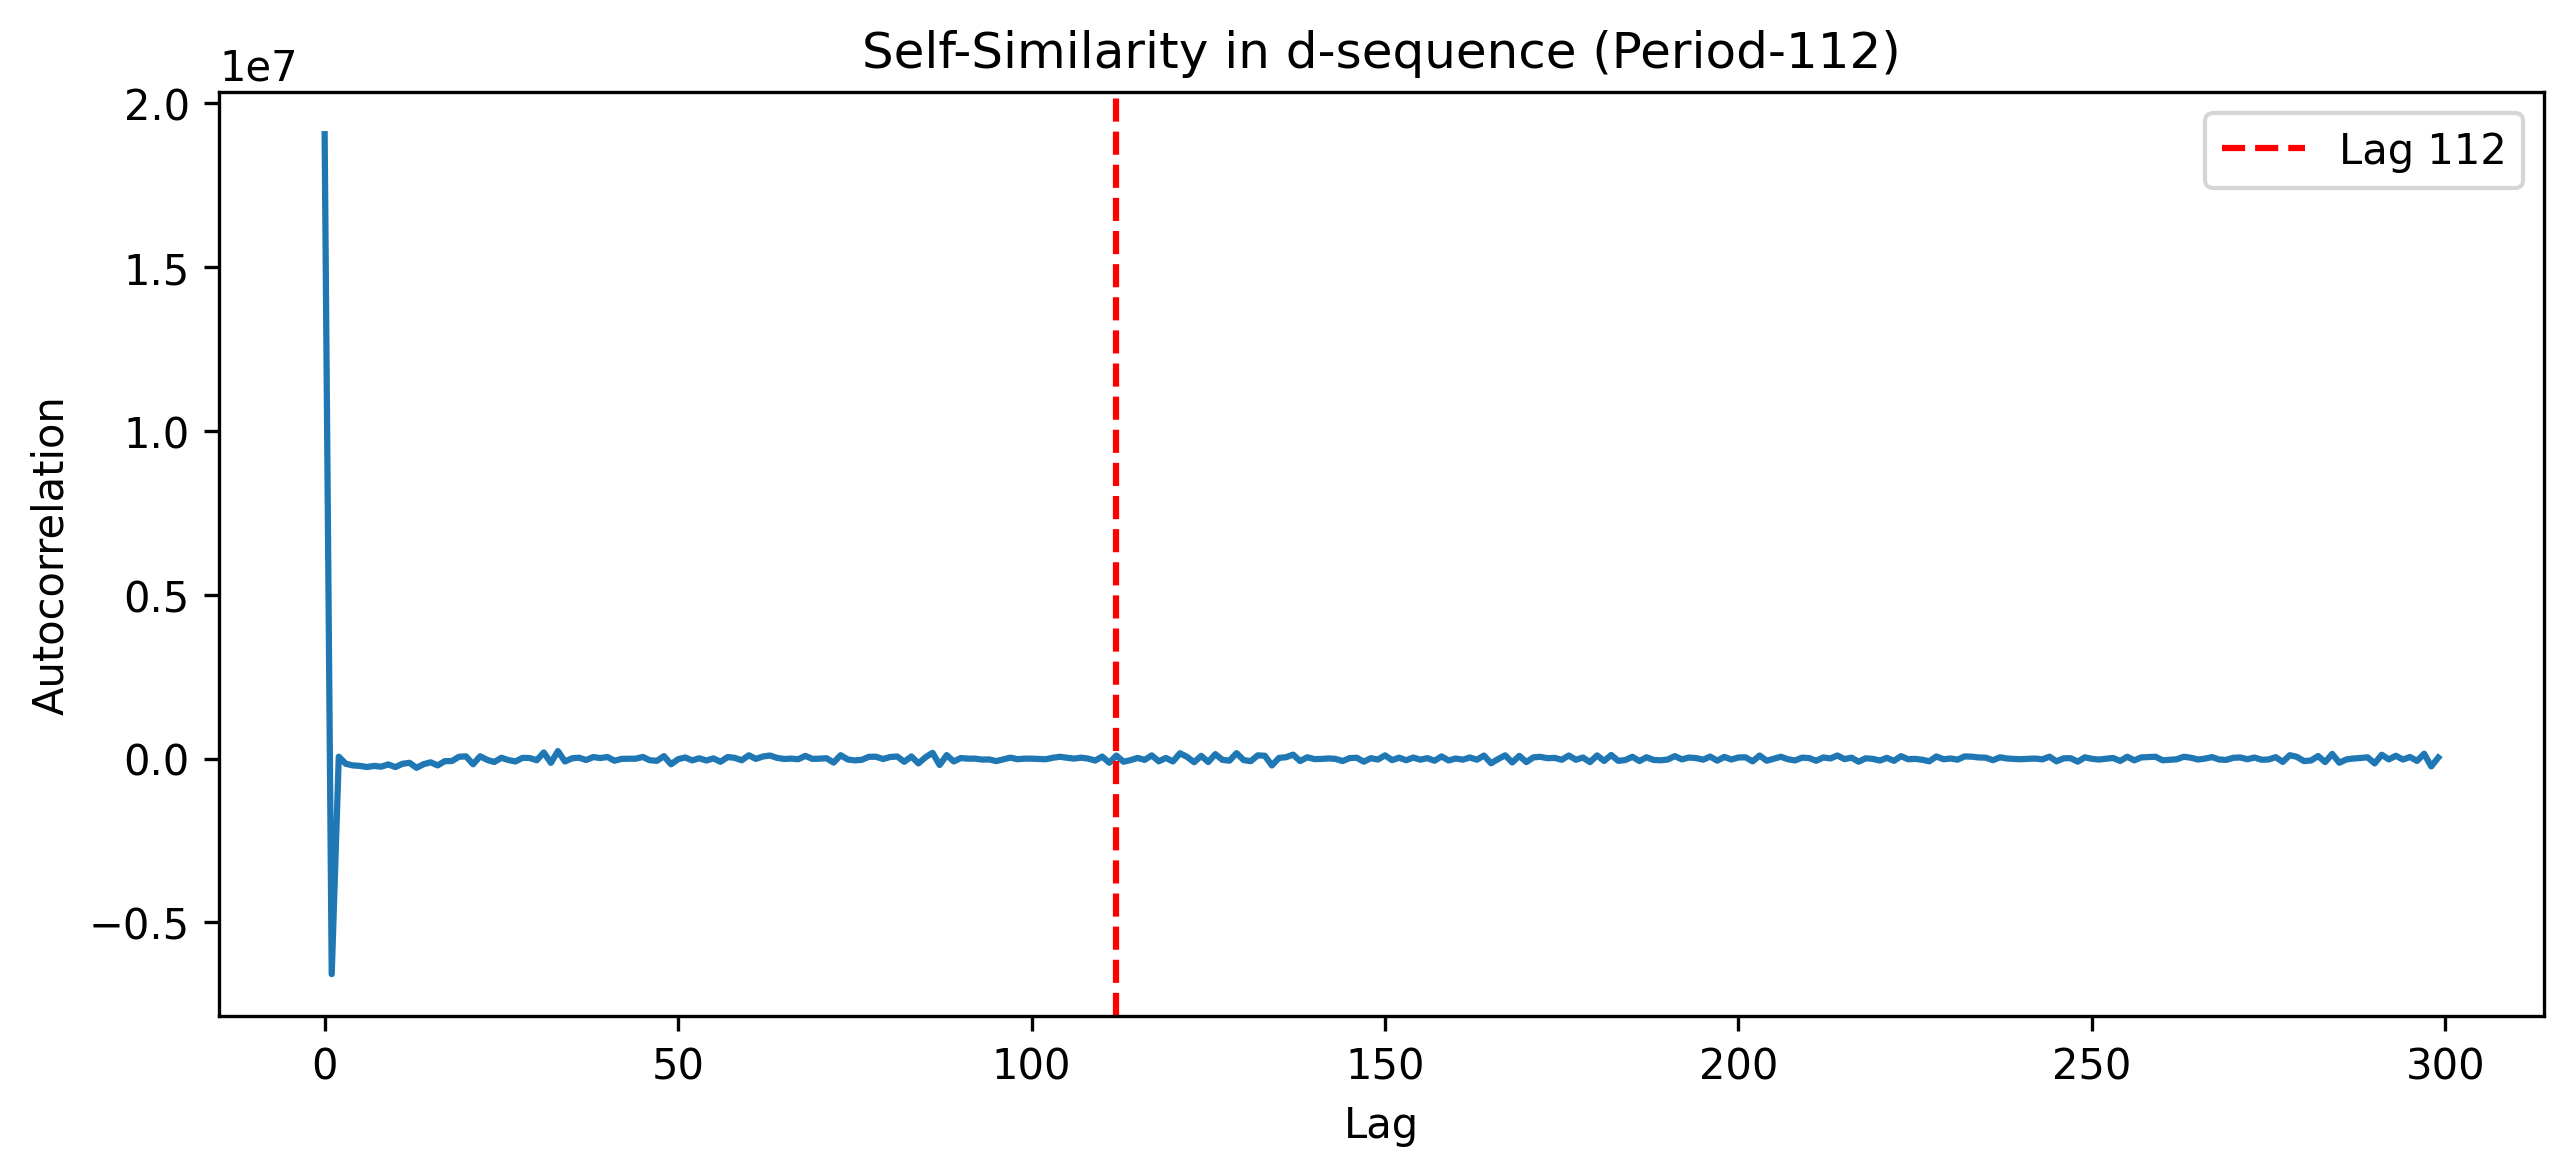
\includegraphics[width=0.85\textwidth]{figures/fig4_autocorrelation.png}
\caption{Autocorrelation of the $d$-value sequence for $n \leq 500$.
         Sharp peak at lag 112 indicates the fundamental modular period.}
\label{fig:autocorr}
\end{figure}

A chi-squared test across multiple moduli confirmed that modulus 112
gives the strongest statistical separation between extending and
non-extending triples ($\chi^2 = 12{,}433$ for mod-112 vs.\
$\chi^2 = 6{,}996$ for mod-56).

\subsection{Conjecture 4: Linear Cone Geometry}

\begin{conjecture}[Linear Cone]
\label{conj:cone}
The set of extending triples $(a,b,c)$ forms a linear cone in
$\mathbb{R}^3$ with asymptotic width
\[
\mathrm{width}(c) \approx \frac{11}{8} \cdot c + f(c \bmod 112),
\]
where $f$ is a bounded periodic function with period $112$.
\end{conjecture}

The slope $11/8 = 1.375$ was estimated from slice-based width
measurements at $c = 5, 10, \ldots, 300$. At each fixed $c$,
the extending triples occupy a contiguous band of $(a,b)$ values
whose width grows linearly in $c$.

%%% SECTION 4: DISCUSSION
\section{Discussion}

\subsection{Comparison with 3\texorpdfstring{$\times$}{x}n Results}

Zeilberger \cite{zeilberger2001} computed $3 \times n$ P-positions
to $n = 130{,}000$ and found apparent linear patterns within families
of positions, but no general formula. Brouwer et al.\ \cite{brouwer2005}
proved that infinitely many winning first moves exist in the third row,
but gave no global characterization.

Our $4 \times n$ results suggest a qualitatively different structure.
The Unique Extension property (Conjecture~\ref{conj:unique}), if true,
would mean the $4$-row game is globally characterized by a function on
triples --- a stronger global statement than anything proven or conjectured
for $3 \times n$ Chomp. The relationship between $3 \times n$ and
$4 \times n$ (every $3 \times n$ P-position extends uniquely, but most
extending triples are $3 \times n$ N-positions) suggests the $4$th row
``rescues'' certain losing $3$-row configurations.

\subsection{Generalization to k\texorpdfstring{$\times$}{x}n}

If the Unique Extension property holds for $4 \times n$, a natural
conjecture is that it generalizes: every $k \times n$ P-position extends
uniquely to a $(k+1) \times n$ P-position. This would imply that all
$k \times n$ Chomp is recursively determined by $2 \times n$ Chomp,
which is fully solved. We regard this as speculative but worth testing
computationally for $k = 5$.

%%% SECTION 5: OPEN QUESTIONS
\section{Open Questions}

\begin{enumerate}
  \item \textbf{Proof of Unique Extension}: Can Conjecture~\ref{conj:unique}
        be proved? A combinatorial or game-theoretic argument explaining
        why the fourth coordinate is uniquely determined would be highly
        significant.

  \item \textbf{Algebraic identity of limits}: Are $L_1, L_2, L_3$
        algebraic numbers? Do they satisfy a common polynomial equation?
        The proximity of $L_3$ to $\cos(3\pi/7)$ is suggestive.

  \item \textbf{Generalization}: Does the Unique Extension property hold
        for $5 \times n$ Chomp? Testing this requires a substantially
        more expensive computation (estimated $O(n^5)$ state space).

  \item \textbf{Origin of period-8}: The period-112 signal decomposes
        as $\mathrm{lcm}(7,8) \times 2$. The factor of 7 is plausibly
        inherited from $3 \times n$ periodicity. What causes the factor
        of 8?

  \item \textbf{Closed-form mask}: Is there a closed-form description
        of the 20\% of triples that extend to $4 \times n$ P-positions?
\end{enumerate}

%%% SECTION 6: REFERENCES
\begin{thebibliography}{9}

\bibitem{berlekamp2001}
E.~Berlekamp, J.~H. Conway, and R.~K. Guy,
\textit{Winning Ways for Your Mathematical Plays}, 2nd ed.,
A K Peters, 2001.

\bibitem{brouwer2005}
A.~E. Brouwer, G.~Horv{\'a}th, and others,
``On three-rowed Chomp,''
\textit{Integers: Electronic Journal of Combinatorial Number Theory},
vol.~5, no.~1, 2005, \#G07.

\bibitem{gale1974}
D.~Gale,
``A curious Nim-type game,''
\textit{American Mathematical Monthly}, vol.~81, pp.~876--879, 1974.

\bibitem{gardner1973}
M.~Gardner,
``Mathematical Games,''
\textit{Scientific American}, January 1973, pp.~110--111.

\bibitem{zeilberger2001}
D.~Zeilberger,
``Three-rowed Chomp,''
\textit{Advances in Applied Mathematics}, vol.~26, pp.~168--179, 2001.

\end{thebibliography}

\end{document}
